\documentclass[progressbar=head]{beamer}
\usetheme{dresden}
\usepackage[utf8]{inputenc}
\usepackage[english]{babel}
\usepackage{amsmath}
\usepackage{amsfonts}
\usepackage{amssymb}
\usepackage{graphicx}

\usepackage{ mathrsfs }

\usepackage{ bbold }

\usepackage{cite}

\usepackage{caption}

% packages
\usepackage{mdframed}

%for links
%\usepackage{hyperref}

% for units
\usepackage{siunitx}

% for the vector on ones
\usepackage{bbm}

% to get the units correctly for printing
%\usepackage{layouts}

% for commenting multiple lines efficiently
\usepackage{comment}

% for fancy tables
\usepackage{booktabs}

%\usepackage{esint}

%\usepackage{mathtools}

%%%%%%%%%%%%%%%%%%%%%%%%%%%%%%%%%%%%%%%%%%%%%%%%%%%%%%%%%%%%%%%%%%%%%%%%%%%%%%%%%%%%%%
%%%%%%%%%%%%%%%%%%%%%%%%%%%%%%%%%%%%%%%%%%%%%%%%%%%%%%%%%%%%%%%%%%%%%%%%%%%%%%%%%%%%%%

\title{New Methods in Electrical Source Imaging Based on EEG and Post-Mortem Pathology Data}
\date{August 7, 2024}
\author{Julio Cesar Enciso-Alva}
\institute{University   of Texas at Arlington}

\newcommand{\bras}[1]{\left\langle #1 \right\rangle}
\newcommand{\pars}[1]{\left( #1 \right)}

%%%%%%%%%%%%%%%%%%%%%%%%%%%%%%%%%%%%%%%%%%%%%%%%%%%%%%%%%%%%%%%%%%%%%%%%%%%%%%%%%%%%%%
%%%%%%%%%%%%%%%%%%%%%%%%%%%%%%%%%%%%%%%%%%%%%%%%%%%%%%%%%%%%%%%%%%%%%%%%%%%%%%%%%%%%%%

%\newcommand{\R}{\mathbb{R}}
\newcommand{\ones}[1]{ \mathbbm{1}_{N_{#1}} \mathbbm{1}_{N_{#1}}^\intercal }
\newcommand{\trans}{^\intercal}

\newcommand{\set}[1]{ \left\{ #1 \right\} }
\newcommand{\ppar}[1]{ \left( #1 \right) }
\newcommand{\spar}[1]{ \left[ #1 \right] }

%\newcommand{\ccon}[2]{\left\phantom{(} #1 \mathrel{}\middle|\mathrel{} #2 \right\phantom{)}}

\DeclareMathOperator*{\argmax}{arg\,max}
\DeclareMathOperator*{\argmin}{arg\,min}

\newcommand{\nnorm}[1]{\lVert #1 \rVert}

\newcommand{\J}{\mathbf{J}}
\newcommand{\Y}{\mathbf{Y}}
\newcommand{\G}{\mathbf{G}}
\newcommand{\U}{\mathbf{U}}
\newcommand{\N}{\mathbf{N}}

\newcommand{\GAM}{\mathbf{\Gamma}}
\newcommand{\SIG}{\mathbf{\Sigma}}
\newcommand{\ga}{\pmb{\gamma}}

\newcommand{\jt}{\mathbf{j}}

\newcommand{\W}{\mathbf{W}}

\newcommand{\id}{\mathbf{I}}
\newcommand{\norm}{\mathcal{N}}

\newcommand{\R}{\mathbb{R}}

\newcommand{\rr}{\mathbf{r}}

%%%%%%%%%%%%%%%%%%%%%%%%%%%%%%%%%%%%%%%%%%%%%%%%%%%%%%%%%%%%%%%%%%%%%%%%%%%%%%%%%%%%%%
%%%%%%%%%%%%%%%%%%%%%%%%%%%%%%%%%%%%%%%%%%%%%%%%%%%%%%%%%%%%%%%%%%%%%%%%%%%%%%%%%%%%%%

\begin{document}

\AtBeginSection[]{
  \begin{frame}
  \vfill
  \centering
  \begin{beamercolorbox}[sep=8pt,center,shadow=true,rounded=true]{title}
    \usebeamerfont{title}\insertsectionhead\par%
  \end{beamercolorbox}
  \vfill
  \end{frame}
}

{
%\metroset{background=dark}
\maketitle

\begin{frame}%{Overview}
\tableofcontents
\end{frame}
}

{
%\metroset{background=dark}
\section{Introduction}
}

\begin{frame}{Electrical Source Imaging Framework}
    The synchronous post-synaptic potentials of multiple neurons generate electrical activity measured by EEG.
    %
    EEG source localization aims to identify the brain regions where these neurons are located.
    
    Electrical Source Imaging assumes that 
    these electrical potential fields
    can be 
    approximated via a finite collection 
    of equivalent dipoles
    with known positions on a grid over the brain.

\begin{figure}
\centering
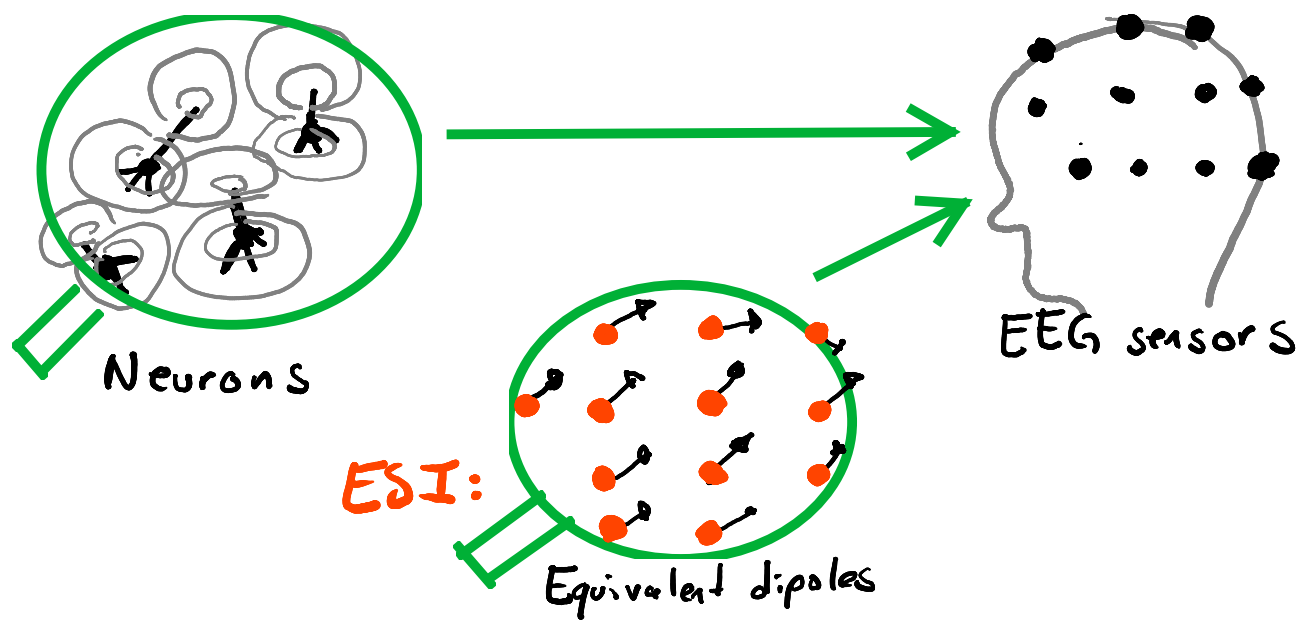
\includegraphics[width=0.6\linewidth]{./img_oldbeamer/sketch03}
\end{figure}
\end{frame}

\begin{frame}{Electrical Source Imaging Framework}
Derivation of ESI methods from physics principles requires relating the \alert{dipoles' magnitude} (from inside the brain) with the \alert{electrical potential field} (at the scalp).
The following derivation is based on 
that of Hallez et al.
\cite{hallez2007review}.

\begin{figure}
\centering
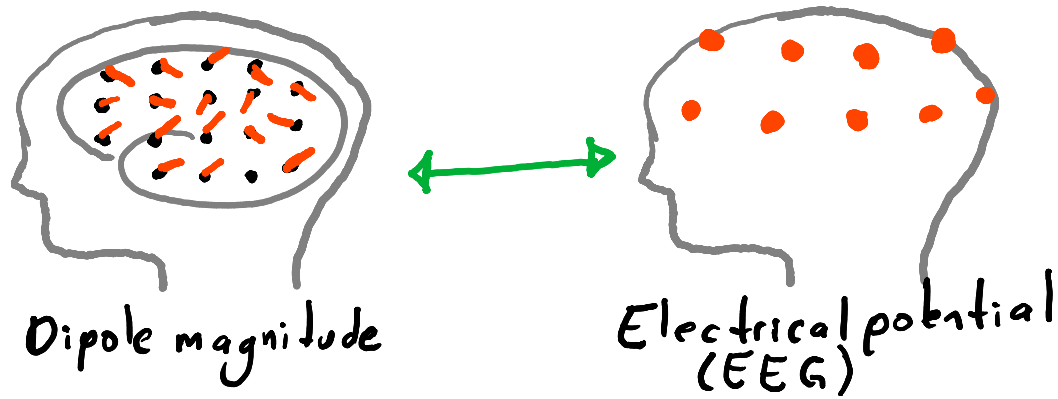
\includegraphics[width=0.75\linewidth]{./img_oldbeamer/sketch04}
\end{figure}
\end{frame}

\begin{frame}{Electrical Source Imaging Framework}
    The modeling of the dipoles starts with the \alert{current density field}, $K: \R^3 \rightarrow \R^3$, whose divergence is defined as
    \begin{equation}
        \nabla \cdot K = \lim_{G \rightarrow 0} \frac{1}{\text{vol}\ppar{G}}
        \oint_{\partial G} K\, dS
    \end{equation}
    In the presence of a single dipole with magnitude $I$, whose source is located at $\rr_{+}$ and whose sink is located at $\rr_{-}$, the divergence of th current density field reduces to
    \begin{equation}
        \nabla \cdot K(\rr) = I \delta\ppar{\rr-\rr_+} - I \delta\ppar{\rr-\rr_-}
        \label{eq:curr_density}
    \end{equation}
\end{frame}

\begin{frame}{Electrical Source Imaging Framework}
From Ohm Law, the \alert{electric field}, $E: \R^3\rightarrow \R^3$, can be obtained as
\begin{equation}
    K = \sigma E
    \label{eq:elec_field}
\end{equation}
with $\sigma: \R^3 \rightarrow \R$ the position-dependent conductivity tensor.
\begin{itemize}
    \item Skull and white matter are known to be anisotropic.
    \item Grey matter, scalp, and cerebrospinal fluid (CSF) are considered isotropic.
\end{itemize}

From quasi-static Maxwell equation $\ppar{\nabla\times E=0}$, the \alert{scalar potential field}, $V: \R^3\rightarrow \R$, can be obtained as
\begin{equation}
    E = - \nabla V
    \label{eq:pot_field}
\end{equation}
\end{frame}

\begin{frame}{Electrical Source Imaging Framework}
From equations \eqref{eq:curr_density}, \eqref{eq:elec_field} and \eqref{eq:pot_field}, the potential field is related to the dipoles according to the following equation
\begin{equation}
\nabla \cdot\ppar{\sigma(\rr)\, \nabla V(\rr) } = 
-I \delta\ppar{\rr-\rr_+} + I \delta\ppar{\rr-\rr_-}
\label{eq:green}
\end{equation}
In this work, equation \eqref{eq:green} is simplified by assuming 
all tissues are isotropic, so $\sigma(\rr)\propto \id$.

Equation \eqref{eq:green} is solved 
only for a finite number of points, 
\begin{equation*}
    \rr = \text{position of EEG sensors at scalp}
\end{equation*}
From the other side, $\rr_\pm$ must be set for the locations of each dipole on the grid.
\end{frame}

\begin{frame}{Electrical Source Imaging Framework}
Equation \eqref{eq:pot_field} must be solved within the whole head volume, which is partitioned into multiple coupled volumes with simplified conductive properties.
Furthermore, in this work, the isotropic case is considered so 
$\sigma(\rr) \propto \id$.

These volumes are typically obtained from an anatomical MRI of the subject or from a template matched to age and gender.

\begin{figure}
\centering
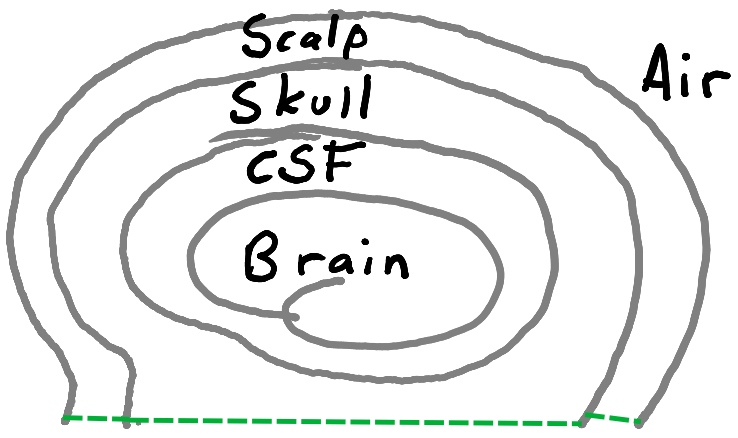
\includegraphics[width=0.4\linewidth]{./img_oldbeamer/sketch06}
\end{figure}
\end{frame}

\begin{frame}{Electrical Source Imaging Framework}
Interface conditions are Neumann, as well as continuity:
\begin{equation}
\left\{
\begin{array}{rl}
    V_1(\rr) \cdot \mathbf{n} &= V_2(\rr) \cdot \mathbf{n} \\
    \ppar{\sigma_1(\rr)\, \nabla V_1(\rr)}\cdot \mathbf{n} &= 
    \ppar{\sigma_2(\rr)\, \nabla V_2(\rr)}\cdot \mathbf{n} \\
    V_1(\rr) &= V_2(\rr)
\end{array}
\right.
\end{equation}
with $\mathbf{n}$ a vector normal to the interface.
For the interface with air, the boundary conditions are different
\begin{equation}
\left\{
\begin{array}{rl}
    V(\rr) \cdot \mathbf{n} &= 0 \\
    \ppar{\sigma(\rr)\, \nabla V(\rr)}\cdot \mathbf{n} &= 0
\end{array}
\right.
\end{equation}    
\end{frame}

\begin{frame}{Electrical Source Imaging Framework}
The location and momentum of each dipole are changed to a more convenient notation.
\begin{align}
\mathbf{d} &= \ppar{I\, p} \mathbf{e}_d \\
\rr_{dip} &= \frac{1}{2}\ppar{\rr_++\rr_-}
\end{align}
where 
$p\, \mathbf{e}_d = \ppar{\rr_+-\rr_-}$, with
with $\mathbf{e}_d$ unitary.
\begin{figure}
\centering
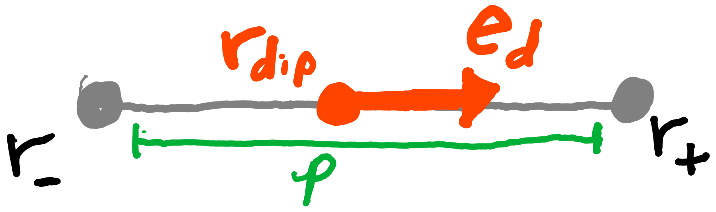
\includegraphics[width=0.4\linewidth]{./img_oldbeamer/sketch05}
\end{figure}
\end{frame}

\begin{frame}{Electrical Source Imaging Framework}
%
Since \eqref{eq:green} is linear, if a dipole $\mathbf{d}$ is decomposed as 
\begin{equation}
\mathbf{d} = d_x \mathbf{e}_x + d_y \mathbf{e}_y + d_z \mathbf{e}_z    
\end{equation}
with $d_x \mathbf{e}_i$ unitary orthogonal vectors, then
\begin{align}
V\ppar{\rr} &=
V\ppar{\rr; \rr_{dip}, \mathbf{d}} 
\nonumber \\
&=
d_x V\ppar{\rr; \rr_{dip}, \mathbf{e}_x} +
d_y V\ppar{\rr; \rr_{dip}, \mathbf{e}_y} +
d_z V\ppar{\rr; \rr_{dip}, \mathbf{e}_z}
\end{align}
For ease of notation, the function $g: \R^{3+3+3}\rightarrow \R$ is defined as
\begin{equation}
    g\ppar{\rr, \rr_{dip}, \mathbf{d}} = V\ppar{\rr; \rr_{dip}, \mathbf{d}}
\end{equation}
\end{frame}

\begin{frame}{Electrical Source Imaging Framework}
Since \eqref{eq:green} is linear, 
by considering $N$ dipoles we can write
\begin{align}
V\ppar{\rr} &=
\sum_{i=1}^N g\ppar{\rr, \rr_{dip_i}, \mathbf{d}_i}
=
\sum_{i=1}^{3N} d_i\, g\ppar{\rr, \rr_{dip_i}, \mathbf{e}_i}
\end{align}
Considering measurements at $M$ locations, this last equation can be arranged as
\begin{equation}
    \begin{bmatrix}
        V\ppar{\rr_1} \\
        \vdots \\
        V\ppar{\rr_M}
    \end{bmatrix}
    =
    \begin{bmatrix}
        g\ppar{\rr_1, \rr_{dip_1}, \mathbf{e}_1}
        &
        \hdots 
        &
        g\ppar{\rr_1, \rr_{dip_{3N}}, \mathbf{e}_{3N}}
        \\
        \vdots & \ddots & \vdots 
        \\
        g\ppar{\rr_M, \rr_{dip_1}, \mathbf{e}_1}
        &
        \hdots 
        &
        g\ppar{\rr_M, \rr_{dip_{3N}}, \mathbf{e}_{3N}}
    \end{bmatrix}
    \begin{bmatrix}
        d_1 \\ \vdots \\ d_{3N}
    \end{bmatrix}
    \label{eq:almost}
\end{equation}
\end{frame}

\begin{frame}{Electrical Source Imaging Framework}
Furthermore, equation \eqref{eq:almost} can be extended trivially to
consider measurements at $M$ locations and $T$ times (indexed from 1 to $T$). The resulting equation can be arranged as
\begin{equation}
    \mathbf{V} = \mathbf{G} \mathbf{D}
    \label{eq:primitive}
\end{equation}
with $\mathbf{V}\in\R^{M\times T}$, $\mathbf{G}\in \R^{M\times 3N}$, $\mathbf{V}\in \R^{3N\times T}$ given by
\begin{align*}
    \mathbf{V}_{m,t} &= V\ppar{\rr_m, t}
    \\
    \mathbf{G}_{n,m} &=
    g\ppar{\rr_m, \rr_{dip_{n}}, \mathbf{e}_{n}}
    \\
    \mathbf{D}_{n,t}
    &=
    d_n(t)
\end{align*}
\end{frame}

\begin{frame}{Electrical Source Imaging Framework}
Notice on equation \eqref{eq:primitive} the matrix $\G$, which is often referred as the \alert{leadfield matrix}, is defined as
\begin{equation*}
    \mathbf{G}_{n,m} =
    g\ppar{\rr_m, \rr_{dip_{n}}, \mathbf{e}_{n}} =
    V\ppar{\rr_m; \rr_{dip_{n}}, \mathbf{e}_{n}}
\end{equation*}
where $V$ is the solution to 
\begin{equation}
\sigma\,
\Delta V(\rr)
= 
-\delta\ppar{\rr-\rr_{dip}-\kappa} + \delta\ppar{\rr-\rr_{dip}+\kappa}
\end{equation}
with the conditions described previously.

This problem is solved numerically either via Boundary Element Method (BEM) with boundaries at the interfaces or via Finite Element Method (FEM).
\end{frame}

{
%\metroset{background=dark}
\section{Literature Review}
}

\begin{frame}{Previous Methods}
%EEG source localization is old in the literature. 
This comparison is focused only on methods based on distributed dipoles. These methods, in general, can be written as
\begin{equation}
    \mathbf{M}^\delta = \mathbf{G} \mathbf{S} + \varepsilon
    \label{eq:general}
\end{equation}
%with 
\begin{itemize}
    \item[$\mathbf{M}$] Matrix of measurements, with noise
    \item[$\mathbf{S}$] Matrix of dipole magnitudes
    \item[$\mathbf{G}$] Leadfield matrix
    \item[$\varepsilon$] Matrix of additive noise at sensors
\end{itemize}

Equation \eqref{eq:general} has been used with %$\mathbf{M}$ 
data from EEG and MEG, and with 
dipoles on either known or unknown orientations
\cite{grech2008review}.

\end{frame}

\begin{frame}{Previous Methods}
Equation \eqref{eq:general} is under-determined and thus doesn't have a unique solution. One common structure is to prioritize the solutions which minimize certain penalty function
\begin{equation}
    \hat{\mathbf{S}} = \argmin_{\mathbf{S}}\, \nnorm{\G \mathbf{S}-\mathbf{M}^\delta} + \lambda\, f\ppar{\mathbf{S}}
    \label{eq:general_min}
\end{equation}
where $f$ is the penalty function, and $\lambda$ is a parameter.

\end{frame}

\begin{frame}{Previous Methods}
    For example, basic Tikhonov regularization considers $f\ppar{\mathbf{S}} = \nnorm{\mathbf{S}}_2^2$.
\begin{equation}
    \hat{\mathbf{S}}_{\text{basic}}
    =
    \G^T \ppar{\G \G^T + \lambda\, \id}^{-1} \mathbf{M}^\delta
\end{equation}

A more general Weighted Minimal Norm Estimator (WMNE) is obtained by considering
$f\ppar{\mathbf{S}} = \nnorm{W\, \mathbf{S}}_2^2$, with $W$ a positive-definite matrix. Then
\begin{equation}
    \hat{\mathbf{S}}_{\text{WMNE}}
    =
    \G^T \ppar{\G \G^T + \lambda\, W^T W}^{\dagger} \mathbf{M}^\delta
\end{equation}
\end{frame}

\begin{frame}{Previous Methods}
LORETA\cite{loreta}  considers 
$f\ppar{\mathbf{S}} = \nnorm{Q\,\overline{\G}\, \mathbf{S}}_2^2$, with $Q$ 
a Laplacian operator and $\overline{\G}$ 
a diagonal matrix
defined as
\begin{align*}
    \overline{\G}_{i,i} &= \nnorm{\G_{\bullet,i}}_2 \\
    Q_{i,j} &=
    \begin{cases}
        1 &\text{if } i=j \\
        -\frac{1}{n} &\text{if } i\in N(i) \\
        0 &\text{otherwise}
    \end{cases}
\end{align*}
with $N(i)$ a neighborhood of $i$ with $n$ grid-points.
%
\begin{equation}
    \hat{\mathbf{S}}_{\text{LORETA}}
    =
    \ppar{\overline{\G}\, Q^T\, Q\,  \overline{\G}}^{-1} \G^T
    \spar{\G \ppar{\overline{\G}\, Q^T\, Q\,  \overline{\G}}^{-1} \G^T}^{\dagger} 
    \mathbf{M}^\delta
\end{equation}
\end{frame}

\begin{frame}{Previous Methods}
sLORETA\cite{sloreta}  considers a small variant of the minimization function
\begin{equation}
    \hat{\mathbf{S}} = \argmin_{\mathbf{S}}\, \nnorm{\G \mathbf{S}-\mathbf{M}^\delta-c \mathbb{1}} + \lambda\, f\ppar{\mathbf{S}}
\end{equation}
with $f\ppar{\mathbf{S}} = \nnorm{\mathbf{S}}_2^2$ and 
$\mathbb{1}=\{1\}^{M\times 1}$.
The solution is given by
\begin{equation}
    \hat{\mathbf{S}}_{\text{sLORETA}}
    =
    \G^T H\spar{H\, \G\, \G^T H+ \lambda H}^{\dagger}
    \mathbf{M}^\delta
\end{equation}
with $H$ an averaging operator constructed as
\begin{equation*}
    H = \id - \ppar{\mathbb{1} \mathbb{1}^T}/\ppar{\mathbb{1}^T \mathbb{1}}
\end{equation*}

\end{frame}

\begin{frame}{Previous Methods}
All the mentioned methods, as well as similar others such as LAURA\cite{LAURA},  FOCUSS\cite{focuss}, among others,
can be interpreted as WMNEs 
specific
weight matrices.

In general, for autonomous\footnote{Penalization is independent of time.} WMNEs, the source estimations can be written as a filter of the observations,
\begin{equation}
    \hat{\mathbf{S}}
    =
    \mathbf{K}\,
    \mathbf{M}^\delta
\end{equation}
with $\mathbf{K}$ known as a \alert{Wiener kernel}.
\end{frame}

\begin{frame}{Previous Methods}
Some selections of the penalty function lead to solutions with desirable properties but not closed-form solutions.

For example, $f(\mathbf{S}) = \nnorm{\mathbf{S}}_1$ can be solved efficiently \cite{review_sparse}, but the solution can't be written as a Wiener Kernel.

The existence of a Wiener Kernel is desirable when the number of dipoles and time points is particularly large. This is the case for long-term monitoring of spontaneous activity.
\end{frame}

\begin{frame}{Previous Results}
Electrical Source Imaging was used; for example, 
in
\cite{dr_pascal}.

\begin{itemize}
\item Glucose transporter type I deficiency (G1D) causes nutrient-responsive epilepsy
\item EEG was recorded for 23 hours following the monitoring
of 6 G1D subjects (ages 2-19)
\item 81 seizures (2-15 minutes) were analyzed
\item ESI was performed using sLORETA
\item ESI results were downsampled in space to the LPA40 anatomical atlas and in time to 20\% segments
\item From 20\% to 40\% of duration, significant changes of relative power (with respect to baseline) were observed to be significant on
the sensorimotor cortex and the thalamus.
\end{itemize}
\end{frame}

\begin{frame}{Previous Results}
\textbf{Note:} ESI methods give the amplitude of electrical activity at any time and space (up to a certain resolution). 
For a 
further clinical analysis,
this data may need to be either downsampled to interpretable units or co-registered between subjects.

\begin{figure}
\centering
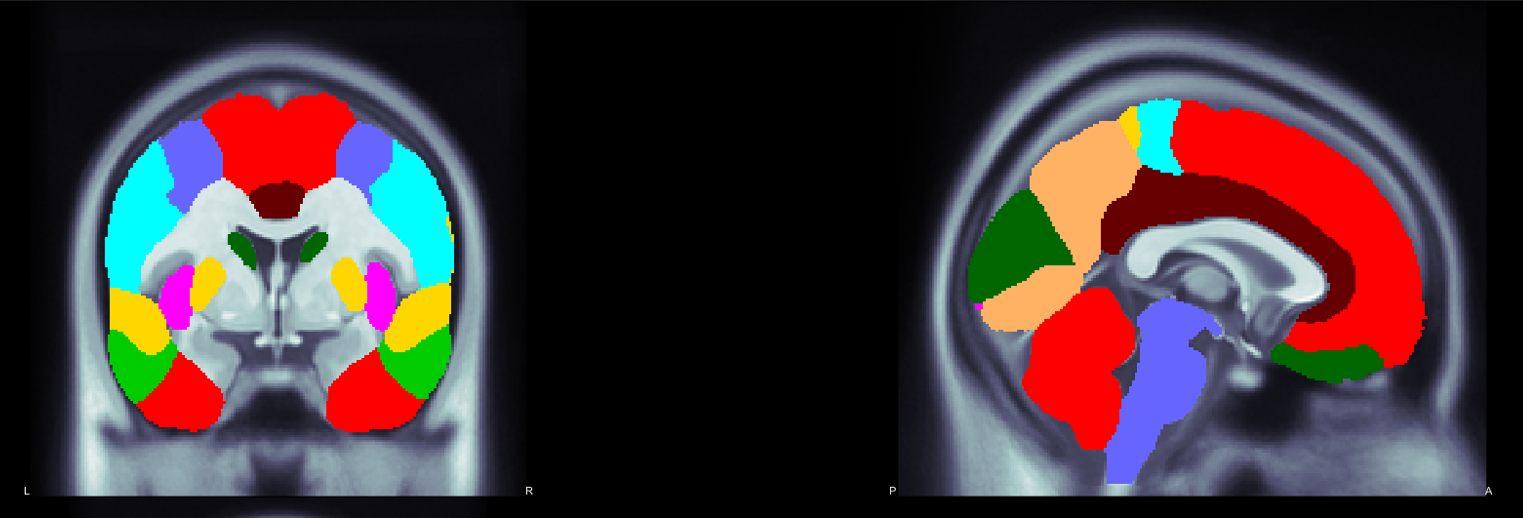
\includegraphics[width=0.9\linewidth]{./img_oldbeamer/MriViewer_Subject02_protocol1_LPBA40_v2}
\end{figure}
\end{frame}

\begin{frame}{Previous Results}
In a separate work\footnote{In preparation}, the quality of ESI estimates is assessed on the presence of 
simultaneous surface- and depth-electrode recordings.
\begin{itemize}
\item In this setup, the recordings of depth electrodes can be interpreted as a
`realistic ground truth'.
\end{itemize}

\begin{figure}
\centering
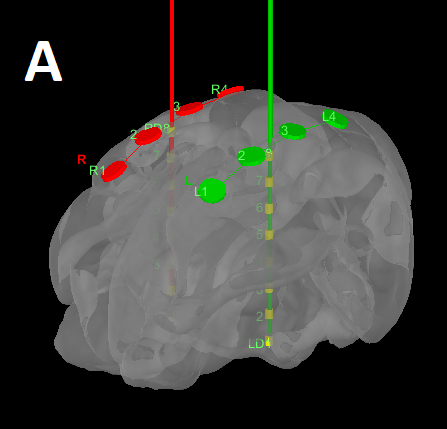
\includegraphics[width=0.35\linewidth]{./img_oldbeamer/positions02_v2}
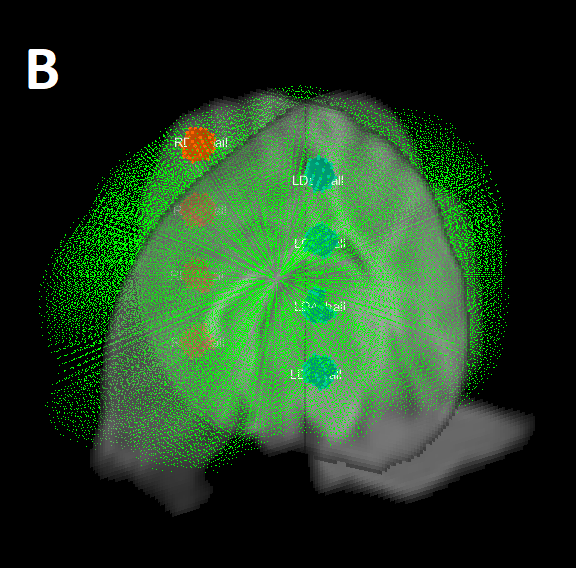
\includegraphics[width=0.35\linewidth]{./img_oldbeamer/positions01_v2}
\end{figure}
\end{frame}

\begin{frame}{Previous Methods for Multimodal Data}
A common framework
to enhance ESI is to incorporate 
`information' from the additional \alert{modalities} of data:
MEG, MRI/fMRI\cite{he2008multimodal, huster2012methods}, PET, fNIRS\cite{fnirs}, etc.
(Figure based on \cite{he2008multimodal}).

\begin{figure}
\centering
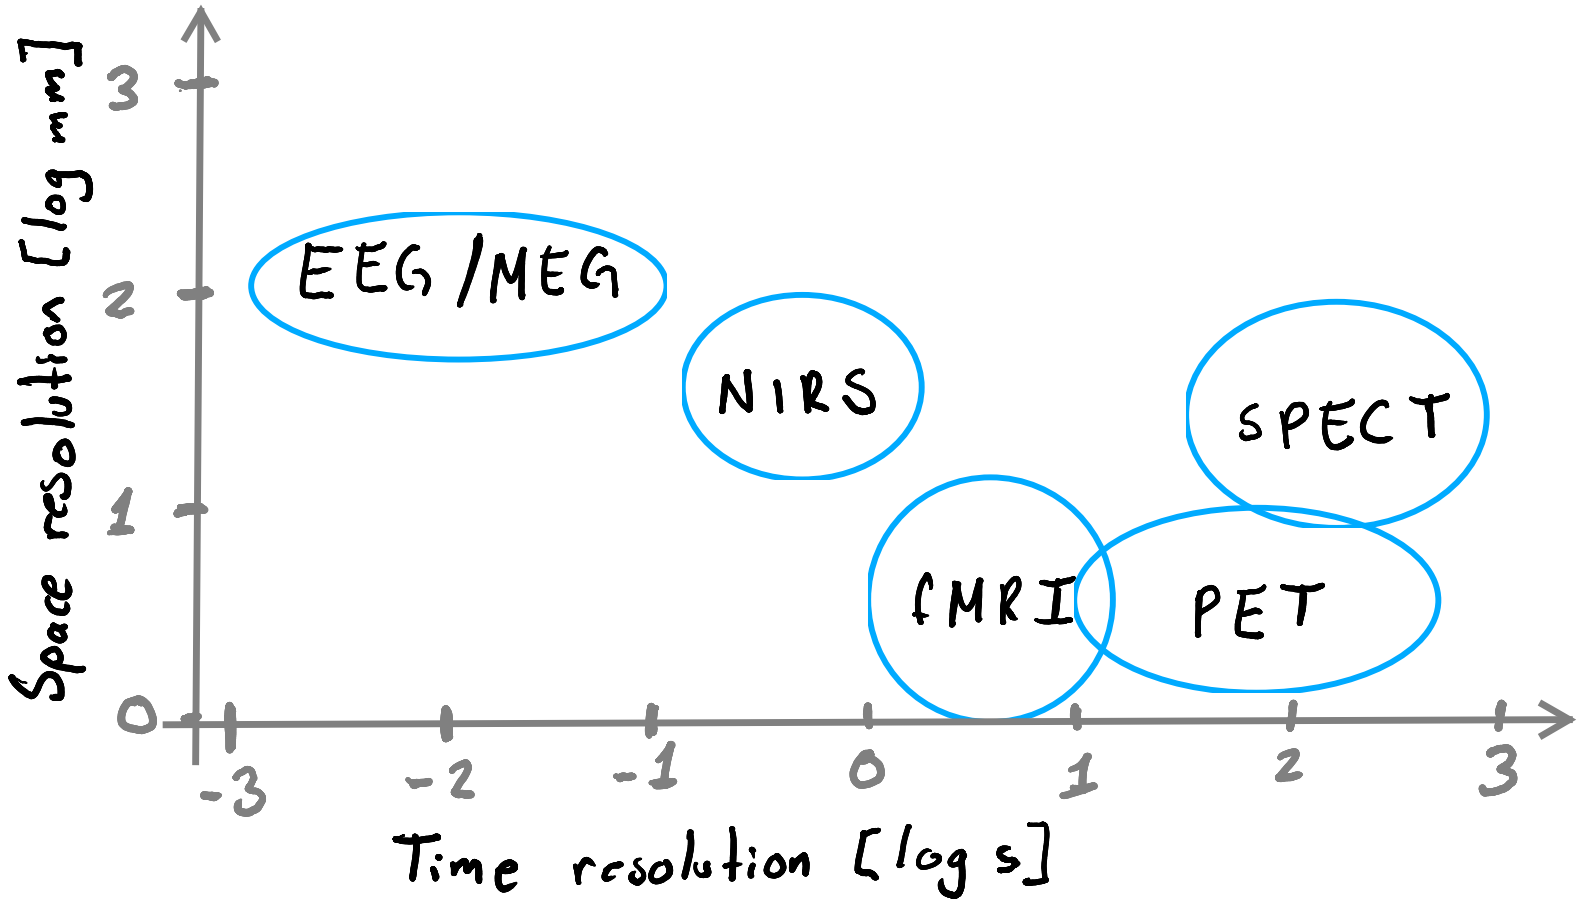
\includegraphics[width=0.65\linewidth]{./img_oldbeamer/sketch07}
\caption{PET=Positron Emission Tomography, NIRS=Near Infrared Spectroscopy, SPECT=Single-Photon Emission Computed Tomography}
\end{figure}
\end{frame}

\begin{frame}{Previous Methods for Multimodal Data}
One big conceptual challenge for multimodal data integration is to model the interaction of the underlying physical phenomena. 
%
Focusing only on unilateral interactions results in asymmetric data integration.

\alert{Asymmetric data fusion} is the extraction of some parameters from one modality, which then are used to further the analysis of the other modality.

Some of the parameters extracted include:
\begin{itemize}
    \item Correlation networks
    \item Statistical Parametric Maps (SPM)
    \item Hidden activation variables \cite{fire}
\end{itemize}

\end{frame}

{
%\metroset{background=dark}
\section{Numerical Experiments}
}

\begin{frame}{A}

\end{frame}

{
%\metroset{background=dark}
\section{Proposed Model}
}

\begin{frame}{Dataset Framework}
The goal is to study the effects of
ischemic stroke of the Middle Cerebral Artery in an animal
model. 
Said lesion is induced.

Electro Corticogram (ECoG) is placed. Recordings start before the lesion and stop 2 hours after it.

In the post-mortem, the brain is stained with
triphenyl-tetrazolium (TTC)
to identify tissues damaged by hypoxia. This information is referred to as \alert{symptoms}.

\begin{figure}
\centering
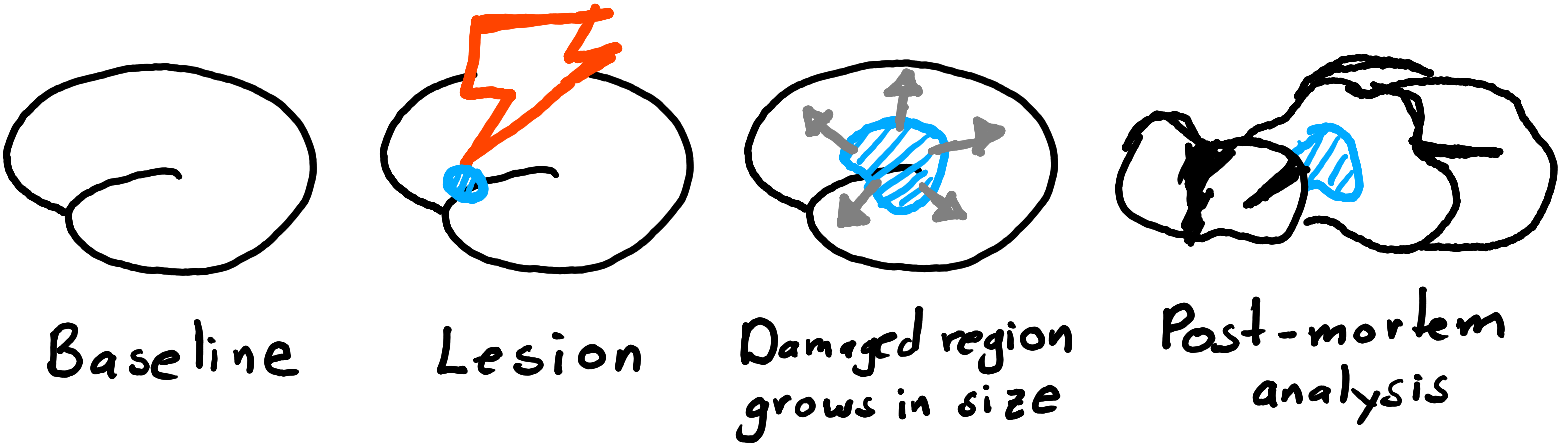
\includegraphics[width=0.8\linewidth]{./img_oldbeamer/sketch01_v2}
\end{figure}
\end{frame}

\begin{frame}{Proposed Work}
The proposed innovation is to use the information from {symptoms} to enhance the results of ESI.
%
A posterior analysis of the results of this ESI may help identify the damaged zone as it evolves over time.

This new model considers two phases:
\begin{enumerate}
    \item Static symptoms (finished, reporting now).
    \item Time-changing symptoms.
\end{enumerate}
\end{frame}



\begin{frame}{Electrical Source Imaging Formulation}
\begin{itemize}
    \item $N$ dipoles with fixed locations on a grid over the brain volume ($<5$ mm between points).
    \item Each dipole is written as the sum of 3 dipoles with canonical orientations and magnitude to be determined.
    \item $M$ EEG sensors at fixed locations over the head surface.
    \item $T$ time-points, labeled from 1 to $T$.
\end{itemize}
\end{frame}

\begin{frame}{Electrical Source Imaging Formulation}
\textbf{Forward problem}, $N$ unconstrained dipoles with fixed locations
\begin{equation}
\Y = \G \J + \varepsilon.
\end{equation}
where
\begin{itemize}
\item $\Y \in \R^{M \times T}$: EEG measurements.
\item $\J \in \R^{3N \times T}$: Dipole magnitudes, 3 dipoles per grid point.
\item $\G \in \R^{3N\times M}$: `Leadfield matrix', originated from the numerical solution of a Poisson PDE on nested media.
\item $\varepsilon\in \R^{M\times T}$: Additive noise at the sensors.
\end{itemize}
\end{frame}

\begin{frame}{Observed symptoms}
The post-mortem observations, referred to as \alert{symptoms}, are registered against a template brain. 

This information is used to label the dipoles in the grid using
${S\in \set{0,1}^{N\times 1}}$, so that $S_n = 1$ if the $n$-th dipole is located on a region where symptoms were observed.

\begin{figure}
\centering
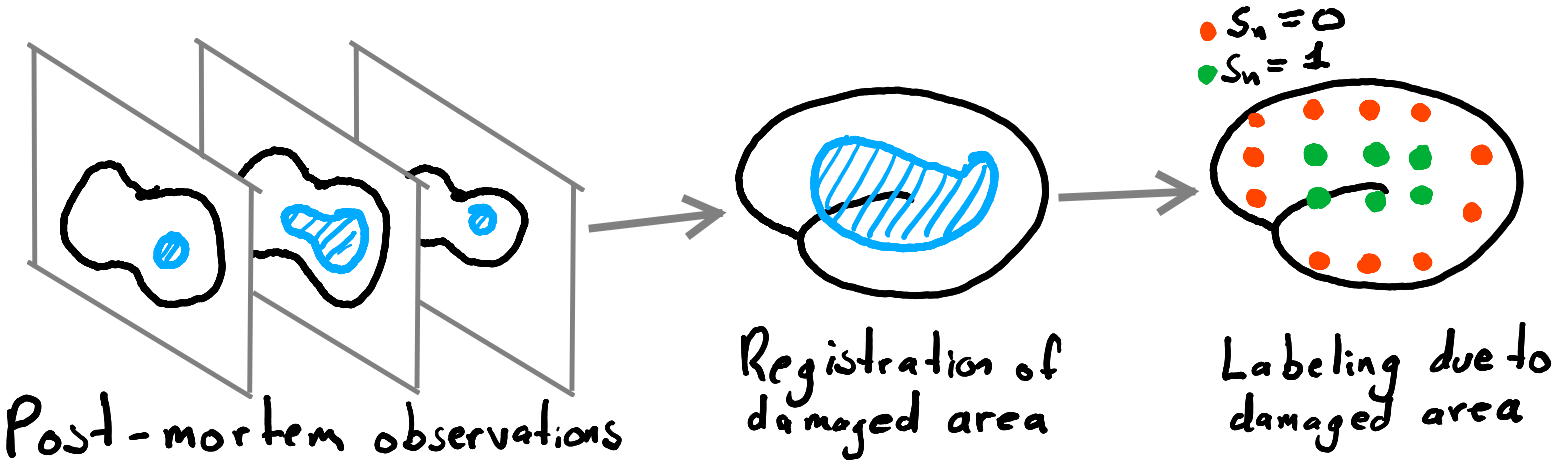
\includegraphics[width=0.8\linewidth]{./img_oldbeamer/sketch02_v2}
\end{figure}

\end{frame}

\begin{frame}{Regional Parcellation}
The brain is divided into $K$ arbitrary regions. The Desikan-Killian anatomical atlas is used for this work.

Let $R_k$ be all the dipoles in the $k$-th region. Define the matrix $L\in \set{0,1}^{N\times K}$ as
\begin{equation}
    L_{n,k} = \begin{cases}
        1, &\text{if } n\in R_k \\
        0, &\text{otherwise.}
    \end{cases}
\end{equation}

\begin{figure}
\centering
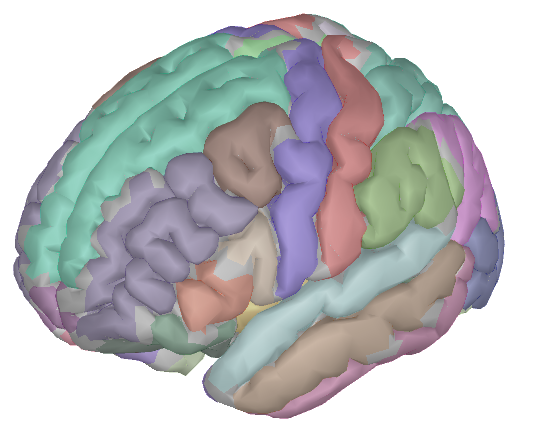
\includegraphics[width=0.3\linewidth]{./img_oldbeamer/desikan}

\end{figure}

\end{frame}

\begin{frame}{Effect of Observed Symptoms}
The relation between symptoms and current density ($\J$) is modeled by adjusting the expected value of the latter based on the symptoms label ($S$).
\begin{equation}
    E\spar{\J_{t,n}} = 
    \begin{cases}
        \U_{t,k} & \text{if } S_n=1 \text{ and } n\in R_k \\
        0 & \text{if } S_n=0
    \end{cases}
\end{equation}

This formulation is equivalent to stating that
\begin{equation}
    \J = \text{diag}\ppar{S} L \U + \N
\end{equation}
where $\mathbf{U}\in \R^{K\times T}$ and $\mathbf{N}\in \R^{N\times T}$ are independent and satisfy
\begin{equation}
    \text{Var}\ppar{\N_{t,n}} \ll \text{Var}\ppar{\U_{t,k}}.
\end{equation}
\end{frame}

\begin{frame}{Distributions from the model}
The proposed model is driven by the following equations
\begin{align}
    \Y &= \G \J + \varepsilon \\
    \J &=  L_S \U + \N
\end{align}
where $\Y, \G$ and $L_S = \text{diag}\ppar{S} L$ are given, and
\begin{align}
    \varepsilon_t &\sim  \norm\ppar{0, \sigma^2 \id } \\
    \N_t &\sim  
    \norm\ppar{0, \gamma_0^2 \id } \\
    \U_t &\sim  
    \norm\ppar{0, \gamma_1^2 \id } 
\end{align}
with $\gamma_0^2 \ll \gamma_1^2$.
\end{frame}

\begin{frame}{Additional assumption}
For simplicity, assume that
the measurements are generated independently over time, so
\begin{equation}
    P\ppar{ \U } = \prod_{t=1}^T P\ppar{ \U_t }
\end{equation}
The analogous holds for $\varepsilon$ and $\N$.
\end{frame}

\begin{frame}{Maximum A Posteriori (MAP) estimator}
The estimator is derived from maximizing the a posteriori probability,
\begin{align}
    \ppar{ \hat{\U}, \hat{\N} } &=
    \argmax_{\U, \N }\,
    \log P\ppar{\ppar{ {\U}, {\N} } \Big| {\Y; \gamma_0, \gamma_2} }
\end{align}
which derives into the following error function
\begin{align}
    F\ppar{ {\U}, {\N};  \gamma_0, \gamma_1} &=
    \frac{1}{2\sigma^2}
    \nnorm{\G L_S \U + \G \N - \Y}_F^2
    \nonumber \\
    &\phantom{=}
    +
    \frac{1}{2\gamma_0^2} \nnorm{\N}_F^2
    +
    \frac{1}{2\gamma_1^2} \nnorm{L_S \U}_F^2
\end{align}
\end{frame}

\begin{frame}{Maximum A Posteriori (MAP) estimator}
    The iterative minimization of the error function can be interpreted as a multi-scale iterative correction
    \begin{align}
        \hat{\N}^{(i+1)} &= \argmin_{\N} F\ppar{\U^{(i)},\N; \gamma_0, \gamma_1}
        \\
        \hat{\U}^{(i+1)} &= \argmin_{\U} F\ppar{\U,\N^{(i)}; \gamma_0, \gamma_1}
    \end{align}
    These steps have the following closed-form
    \begin{align}
        \hat{\N}^{(i+1)} &=
        \hat{\N}^{(i)}
        -
        \G^T \spar{\G \G^T + \frac{\gamma_0^2}{\sigma^2} \id}^{-1} L_S \ppar{\hat{\U}^{(i)}-\hat{\U}^{(i-1)} }
        \\
        \hat{\U}^{(i+1)} &=
        \hat{\U}^{(i)}
        -
        L_S^T \G^T \spar{\G L_S L_S^T \G^T + \frac{\gamma_1^2}{\sigma^2} \id}^{-1} \ppar{\hat{\N}^{(i)}-\hat{\N}^{(i-1)} }
    \end{align}
\end{frame}

{
%\metroset{background=dark}
\subsection{Derivation of the Estimator}
}

\begin{frame}
\begin{align*}
    \ppar{ \hat{\U}, \hat{\N} } &=
    \argmax_{\U, \N }\,
    \log P\ppar{\ppar{ {\U}, {\N} } \Big| {\Y; \gamma_0, \gamma_2} }
    \\
    &=
    \argmax_{\U, \N }\, \sum_{t=1}^T 
    \log P\ppar{\ppar{ {\U_t}, {\N_t} } \Big| {\Y_t; \gamma_0, \gamma_2} }
    \\
    &=
    \argmax_{\U, \N }\, \sum_{t=1}^T  \left[
    \log P\ppar{{ \Y_t } \Big| { \ppar{\U_t, \N_t}  ; \gamma_0, \gamma_2} }
    \right.
    \\
    &\phantom{=}
    \left.
    +
    P\ppar{{ {\U_t}  ; \gamma_0, \gamma_2} }
    +
    P\ppar{{ {\N_t}  ; \gamma_0, \gamma_2} }
    \right]
    \\
    &=
    \argmax_{\U, \N }\, \sum_{t=1}^T  \left[
    -\frac{1}{2\sigma^2}
    \nnorm{\G L_S \U_t + \G \N_t - \Y_t}_2^2
    \right.
    \\
    &\phantom{=}
    \left.
    -
    \frac{1}{2\gamma_0^2} \nnorm{\N_t}_2^2
    -
    \frac{1}{2\gamma_1^2} \nnorm{L_S \U_t}_2^2
    \right]
\end{align*}
\end{frame}

\begin{frame}
\begin{align*}
\ppar{ \hat{\U}, \hat{\N} } 
&=
    \argmax_{\U, \N }\, \sum_{t=1}^T  \left[
    -\frac{1}{2\sigma^2}
    \nnorm{\G L_S \U_t + \G \N_t - \Y_t}_2^2
    \right.
    \\
    &\phantom{=}
    \left.
    -
    \frac{1}{2\gamma_0^2} \nnorm{\N_t}_2^2
    -
    \frac{1}{2\gamma_1^2} \nnorm{L_S \U_t}_2^2
    \right]
    \\
    &=
    \argmax_{\U, \N }\, \left[
    -\frac{1}{2\sigma^2}
    \nnorm{\G L_S \U + \G \N - \Y}_F^2
    \right.
    \\
    &\phantom{=}
    \left.
    -
    \frac{1}{2\gamma_0^2} \nnorm{\N}_F^2
    -
    \frac{1}{2\gamma_1^2} \nnorm{L_S \U}_F^2
    \right]
\end{align*}
\end{frame}

\begin{frame}
This derives into the following error function
\begin{align*}
    F\ppar{ {\U}, {\N};  \gamma_0, \gamma_1} &=
    \frac{1}{2\sigma^2}
    \nnorm{\G L_S \U + \G \N - \Y}_F^2
    \nonumber \\
    &\phantom{=}
    +
    \frac{1}{2\gamma_0^2} \nnorm{\N}_F^2
    +
    \frac{1}{2\gamma_1^2} \nnorm{L_S \U}_F^2
\end{align*}
So that
\begin{align*}
\ppar{ \hat{\U}, \hat{\N} } 
&=
    \argmin_{\U, \N }\, F\ppar{ {\U}, {\N};  \gamma_0, \gamma_1}
\end{align*}
Notice that the function is convex in both $\U$ and $\N$, and thus it can be minimized iteratively over it's arguments,
    \begin{align*}
        \hat{\N}^{(i+1)} &= \argmin_{\N} F\ppar{\U^{(i)},\N; \gamma_0, \gamma_1}
        \\
        \hat{\U}^{(i+1)} &= \argmin_{\U} F\ppar{\U,\N^{(i)}; \gamma_0, \gamma_1}
    \end{align*}
\end{frame}

\begin{frame}
Minimization is carried away via Lagrange multipliers with the constraint $\G L_S \U + \G \N - \Y=0$.
\begin{align*}
    \hat{\N}^{(i+1)} &= \argmin_{\N}  F\ppar{\U^{(i)},\N; \gamma_0, \gamma_1}
    \\
    &\phantom{=}
    \quad \quad
    \text{st} \quad \quad
    \G L_S \U^{(i)} + \G \N - \Y=0
\end{align*}
This leads to the Lagrangian function
\begin{align*}
    \mathscr{L}_\N \ppar{\N, \lambda; \U^{(i)}, \gamma_0}
    &=
    \frac{1}{2\sigma^2}
    \nnorm{\G L_S \U^{(i)} + \G \N - \Y}_F^2
    +
    \frac{1}{2\gamma_0^2} \nnorm{\N}_F^2
    \\
    &\phantom{=}
    +\lambda^T\ppar{\G L_S \U^{(i)} + \G \N - \Y}
\end{align*}
\end{frame}

\begin{frame}
\begin{align*}
\frac{\partial}{\partial \N}
\mathscr{L}_\N \ppar{\N, \lambda; \U^{(i)}, \gamma_0}
    &=
    \frac{1}{\sigma^2}
    \G^T
    \ppar{\G L_S \U^{(i)} + \G \N - \Y}
    \\
    &\phantom{=}
    +
    \frac{1}{\gamma_0^2} {\N}
    +
    \G^T \lambda
    \\
    \frac{\partial}{\partial \lambda} 
    \mathscr{L}_\N \ppar{\N, \lambda; \U^{(i)}, \gamma_1}
    &=
    \G L_S \U^{(i)} + \G \N - \Y
\end{align*}
By setting $\frac{\partial}{\partial \N} \mathscr{L}_\N = 0$ and 
$\frac{\partial}{\partial \lambda} \mathscr{L}_\N = 0$, it arises the conditions
\begin{align*}
    {\frac{1}{\gamma_0^2} { \N}
    +
    \G^T \lambda} &= 0
    \\
    \G \N 
    &= \Y - \G L_S \U^{(i)} 
\end{align*}
\end{frame}

\begin{frame}
\begin{align*}
&&
{\frac{1}{\gamma_0^2} { \N}
    +
    \G^T \lambda} &= 0
\\
\Rightarrow
&&
\N &= -\gamma_0^2 \G^T \lambda
\\
\Rightarrow
&&
-\gamma_0^2 \G \G^T \lambda
&=
\Y - \G L_S \U^{(i)} 
\\
\Rightarrow
&&
\lambda &=
-\frac{1}{\gamma_0^2} \spar{\G \G^T+ \frac{\gamma_0^2}{\sigma^2}^{-1}}^{-1} \ppar{\Y - \G L_S \U^{(i)} }
\\
\Rightarrow
&&
\N &=
\G^T \spar{\G \G^T+ \frac{\gamma_0^2}{\sigma^2}^{-1}} \ppar{\Y - \G L_S \U^{(i)} }
\end{align*}
Thus, concluding the following
\begin{align*}
\N^{(i+1)} &=
\G^T \spar{\G \G^T+ \frac{\gamma_0^2}{\sigma^2}^{-1}} \ppar{\Y - \G L_S \U^{(i)} }
\end{align*}
\end{frame}

\begin{frame}{Maximum A Posteriori (MAP) estimator}
For the iterative step, consider the following,
\begin{align*}
\N^{(i+1)} &=
\G^T \spar{\G \G^T+ \frac{\gamma_0^2}{\sigma^2}^{-1}} \ppar{\Y - \G L_S \U^{(i)} }
\\
\N^{(i)} &=
\G^T \spar{\G \G^T+ \frac{\gamma_0^2}{\sigma^2}^{-1}} \ppar{\Y - \G L_S \U^{(i-1)} }
\\
\Rightarrow
\N^{(i+1)}-\N^{(i)} &=
\G^T \spar{\G \G^T+ \frac{\gamma_0^2}{\sigma^2}^{-1}} \G L_S \ppar{ \U^{(i)}-\U^{(i-1)} }
\end{align*}
\end{frame}

\begin{frame}{Maximum A Posteriori (MAP) estimator [repeated slide]}
    The iterative minimization of the error function can be interpreted as a multi-scale iterative correction
    \begin{align}
        \hat{\N}^{(i+1)} &= \argmin_{\N} F\ppar{\U^{(i)},\N; \gamma_0, \gamma_1}
        \\
        \hat{\U}^{(i+1)} &= \argmin_{\U} F\ppar{\U,\N^{(i)}; \gamma_0, \gamma_1}
    \end{align}
    These steps have the following closed-form
    \begin{align}
        \hat{\N}^{(i+1)} &=
        \hat{\N}^{(i)}
        -
        \G^T \spar{\G \G^T + \frac{\gamma_0^2}{\sigma^2} \id}^{-1} L_S \ppar{\hat{\U}^{(i)}-\hat{\U}^{(i-1)} }
        \\
        \hat{\U}^{(i+1)} &=
        \hat{\U}^{(i)}
        -
        L_S^T \G^T \spar{\G L_S L_S^T \G^T + \frac{\gamma_1^2}{\sigma^2} \id}^{-1} \ppar{\hat{\N}^{(i)}-\hat{\N}^{(i-1)} }
    \end{align}
\end{frame}

\begin{frame}{Special cases}
In the special case with only one region, the proposed model is equivalent to widely known models:
\begin{itemize}
\item If the region has no symptoms, the model reduces to a Tikhonov penalization.
\item If the region has symptoms, the model reduces to sLORETA.
\end{itemize}
\end{frame}


{
%\metroset{background=dark}
\subsection{Numerical Experiments}
}

\begin{frame}{Numerical experiments}
Synthetic data is simulated with one source at a known location at different SNR levels. 
\begin{figure}
\centering
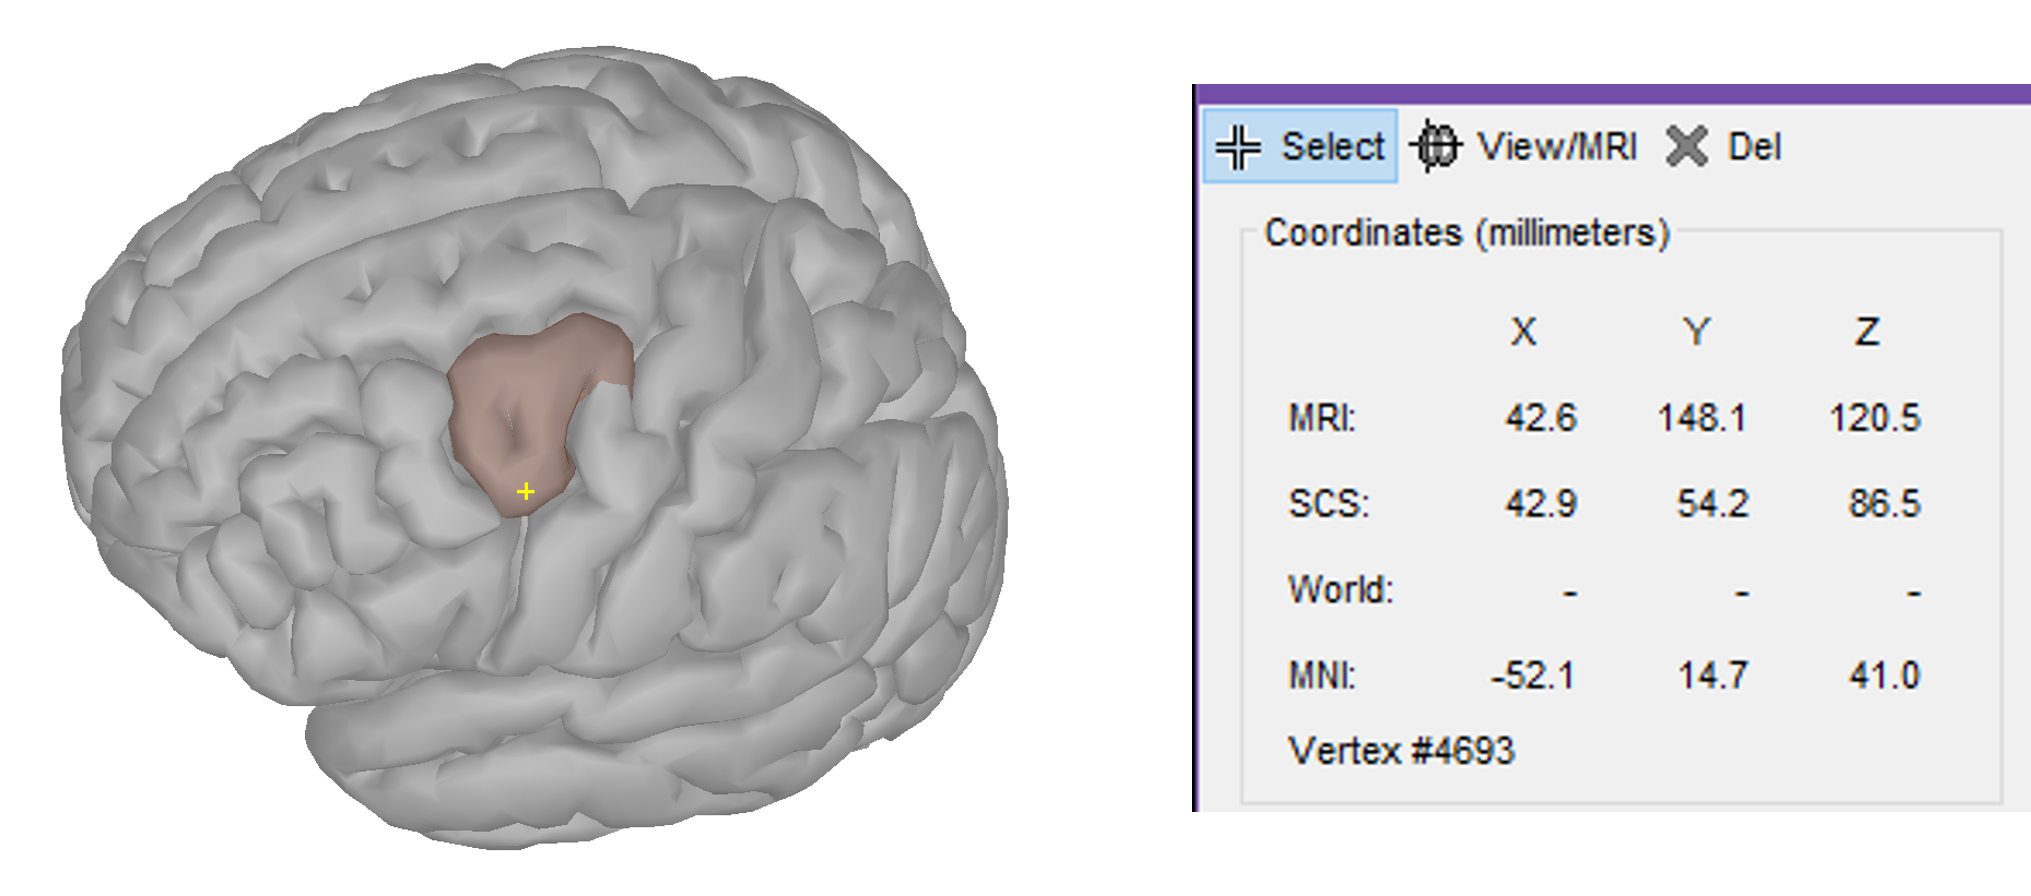
\includegraphics[width=0.8\linewidth]{./img_oldbeamer/protocol1}
\end{figure}
\end{frame}

\begin{frame}{SNR = 10}
Left to right: Classic Tikhonov, sLORETA, proposed method
\begin{figure}
\centering
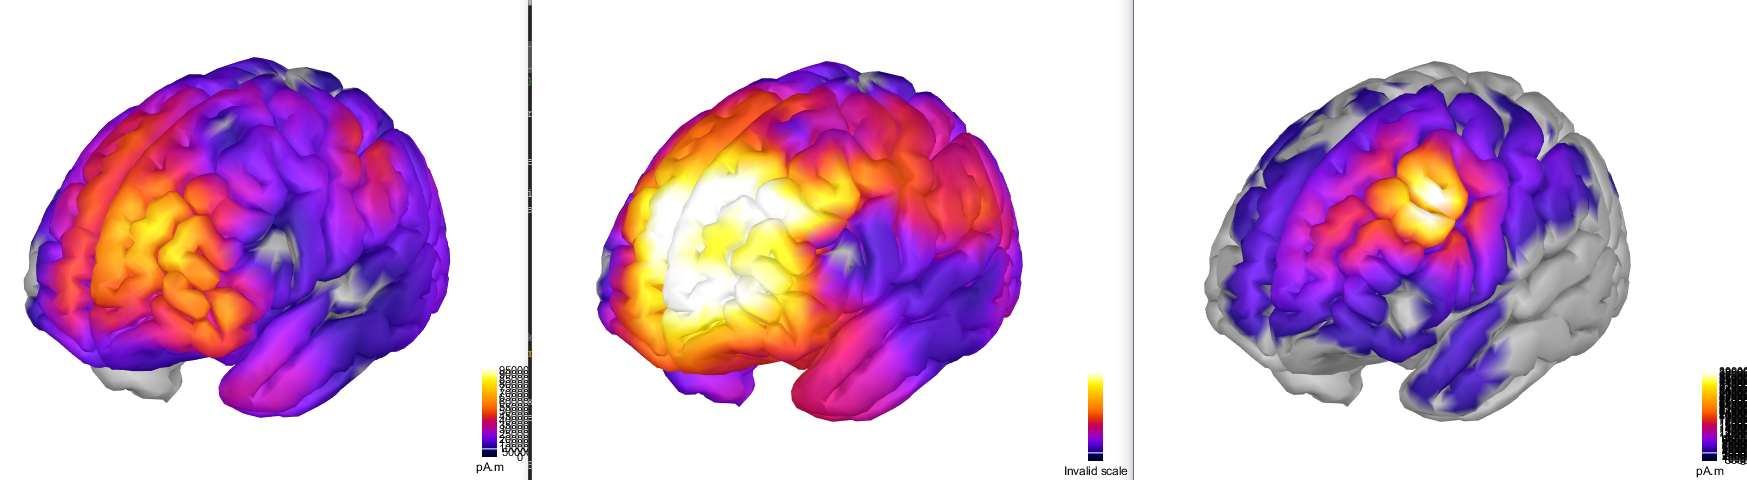
\includegraphics[width=1\linewidth]{./img_oldbeamer/comparison1}
\end{figure}
\end{frame}


{
%\metroset{background=dark}
\subsection{Future Work}
}

\begin{frame}{Future work}
\begin{itemize}
    \item The implemented method expands over previous methods for ESI by incorporating information from binary symptoms observed in the brain.
    \item As a first phase, these binary symptoms are assumed to be static over time. However, there is enough physiological information to claim that the damaged area grows over time.
    \item This time-changing damaged area can be incorporated into the model by including a time-changing vector of symptoms, ${S\in \set{0,1}^{N\times T}}$.
\end{itemize}
\end{frame}

\begin{frame}{Future work}
The following equations drive the proposed new model
\begin{align}
    \Y &= \G \J + \varepsilon \\
    \J_t &=  L_{S_t} \U_t + \N_t
\end{align}
where $\Y, \G$ and $L_{S_t} = \text{diag}\ppar{S_t} L$ are given, and
\begin{align}
    \varepsilon_t &\sim  \norm\ppar{0, \sigma^2 \id } \\
    \N_t &\sim  
    \norm\ppar{0, \gamma_0^2 \id } \\
    \U_t &\sim  
    \norm\ppar{0, \gamma_1^2 \id } 
\end{align}
with $\gamma_0^2 \ll \gamma_1^2$.
\end{frame}

\begin{frame}{Thanks for your attention}

\end{frame}

{
%\metroset{background=dark}
\section{Bibliography}
}

\begin{frame}[allowframebreaks]
        \frametitle{References}
\bibliographystyle{abbrv} % We choose the "plain" reference style
\bibliography{./refs_old} % Entries are in the refs.bib file
\end{frame}

\end{document}